\epigraph{The difference between ideas and reality is the
difference between philosophy and engineering. The work to transform one into
the other is scientific research}{{\itshape V-Research}}
\begin{figure}[t]
	\centering
	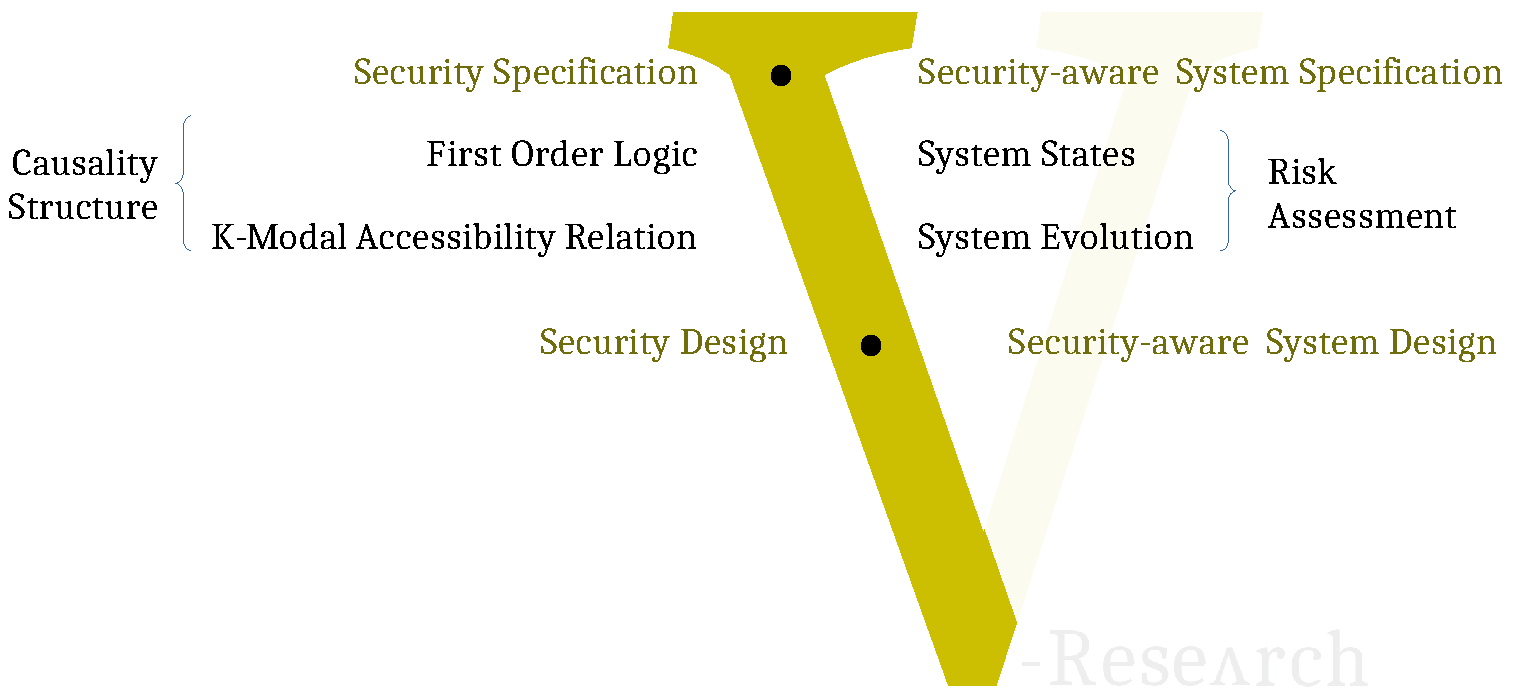
\includegraphics[width=\textwidth]{vmodel.pdf}
	\caption{Cybersecurity Engineering Life-cycle}
	\label{fig:knowledge-belief}
\end{figure}

\subsubsection{Relevant Standards}\label{sec:standards}
\begin{enumerate}[noitemsep]
	\item DO-326A
\end{enumerate}

\begin{enumerate}
\item specification -- definition of the desired design of a system. The
specification is verified w.r.t. the  $\abf$ theory. Checking the
controls of the whole cybersecurity life-cycle and the relation with
CWE.
\item design -- the mitigations identified in the specification stage
are implemented into the design. The security of the assets w.r.t. the design are
verified with a, so called, cybersecurity risk assessment.
\end{enumerate}
